\begin{figure*}
       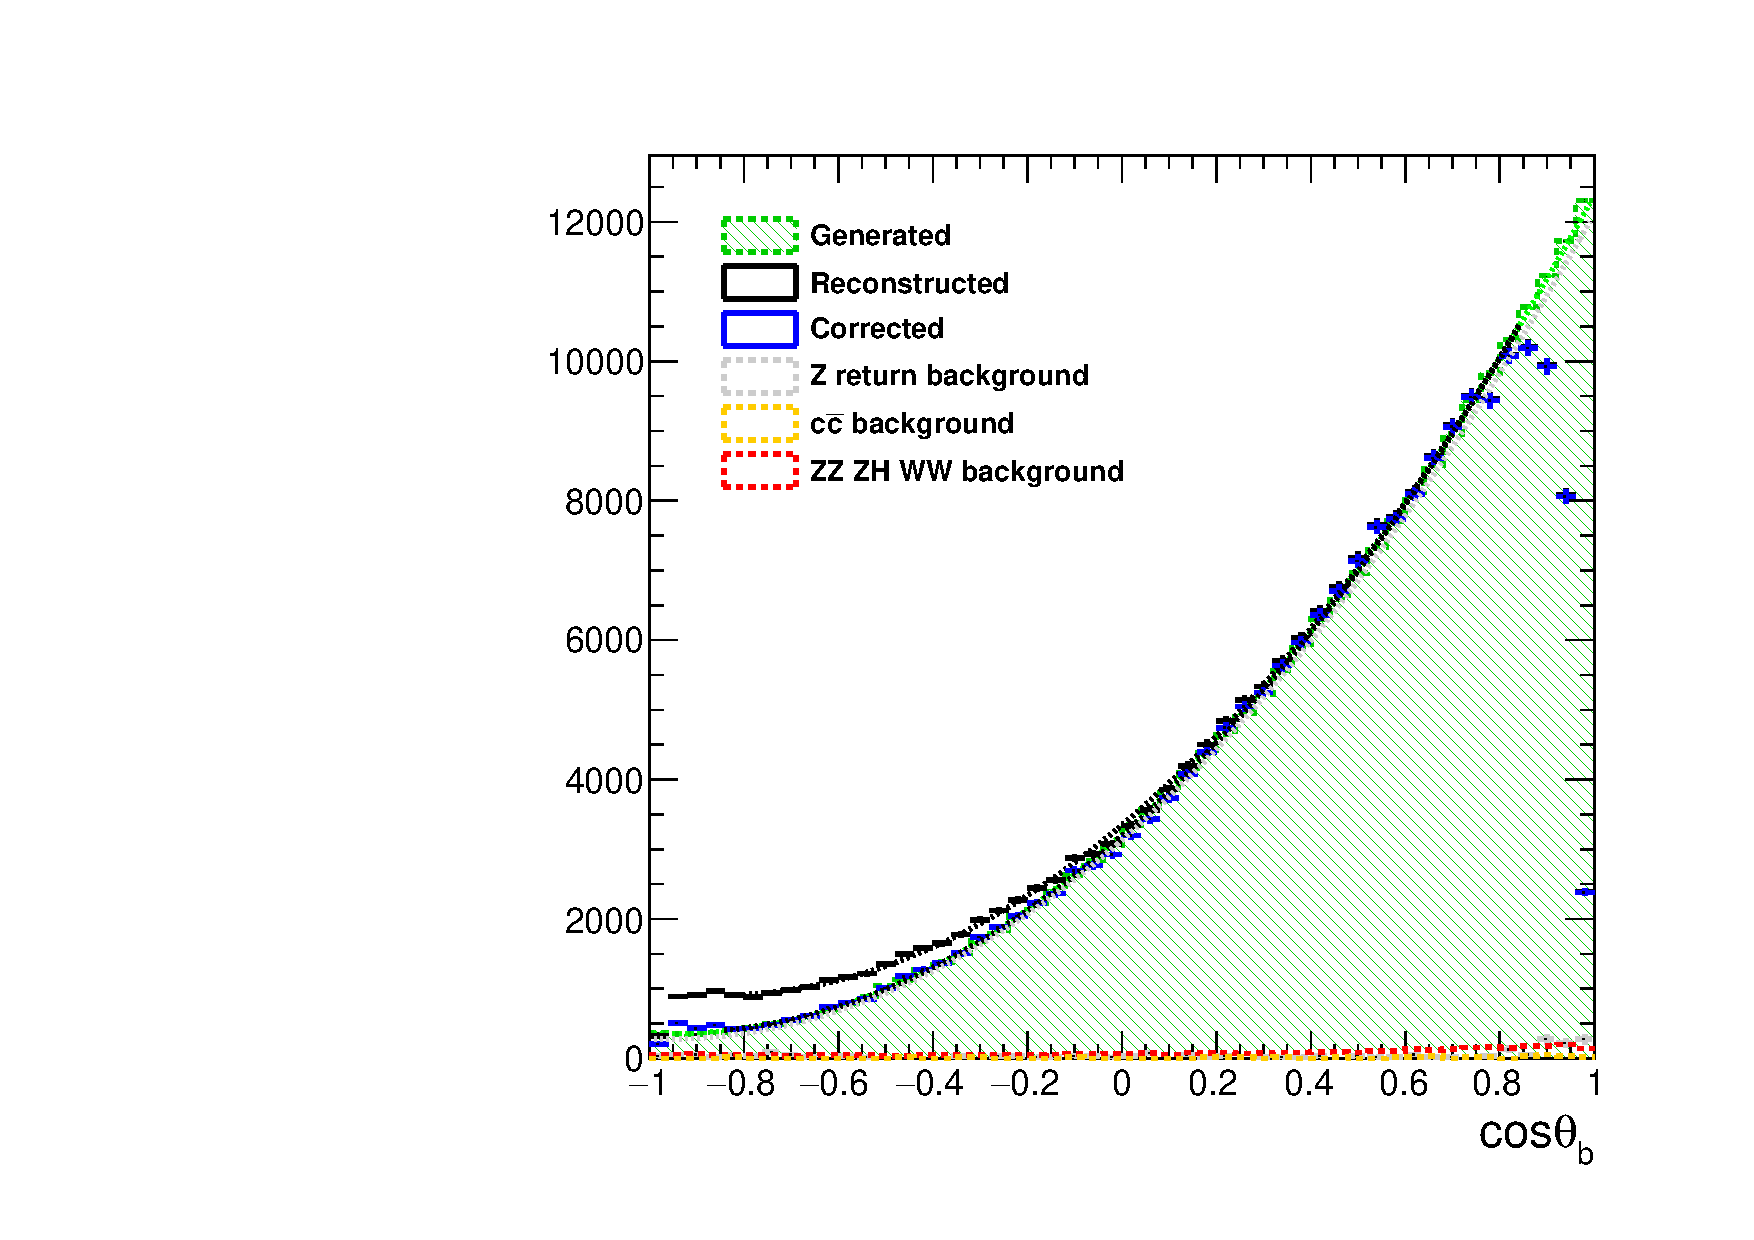
\includegraphics[width=0.45\linewidth]{./chapters/figures/basymmetry-final-left.pdf}
       \llap{\shortstack{%
                       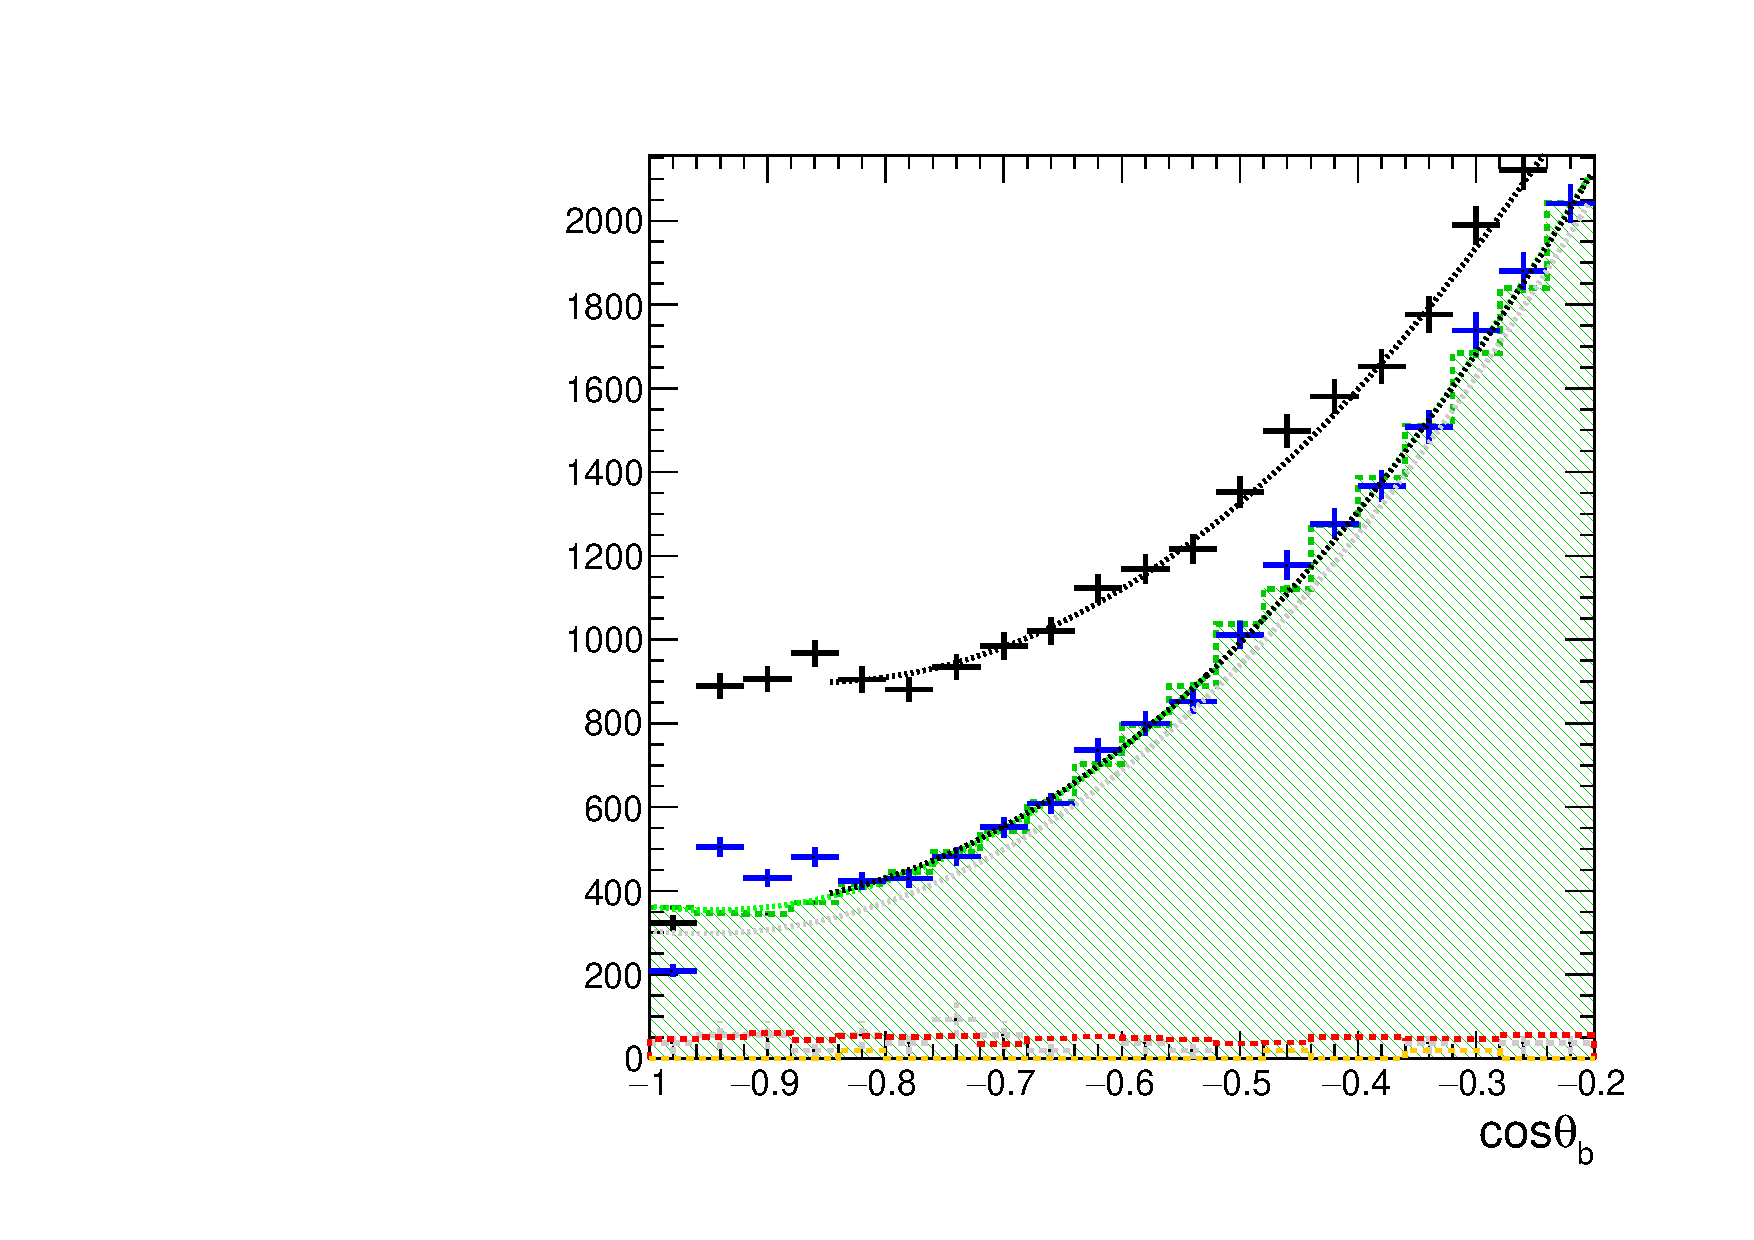
\includegraphics[clip, trim=0cm 0cm 1.8cm 1.7cm, scale=.15]{./chapters/figures/zoom-final.pdf}\\
                       \rule{0ex}{0.67in}%
               }
               \rule{2.2in}{0ex}}
        \hspace{0.2cm}       
        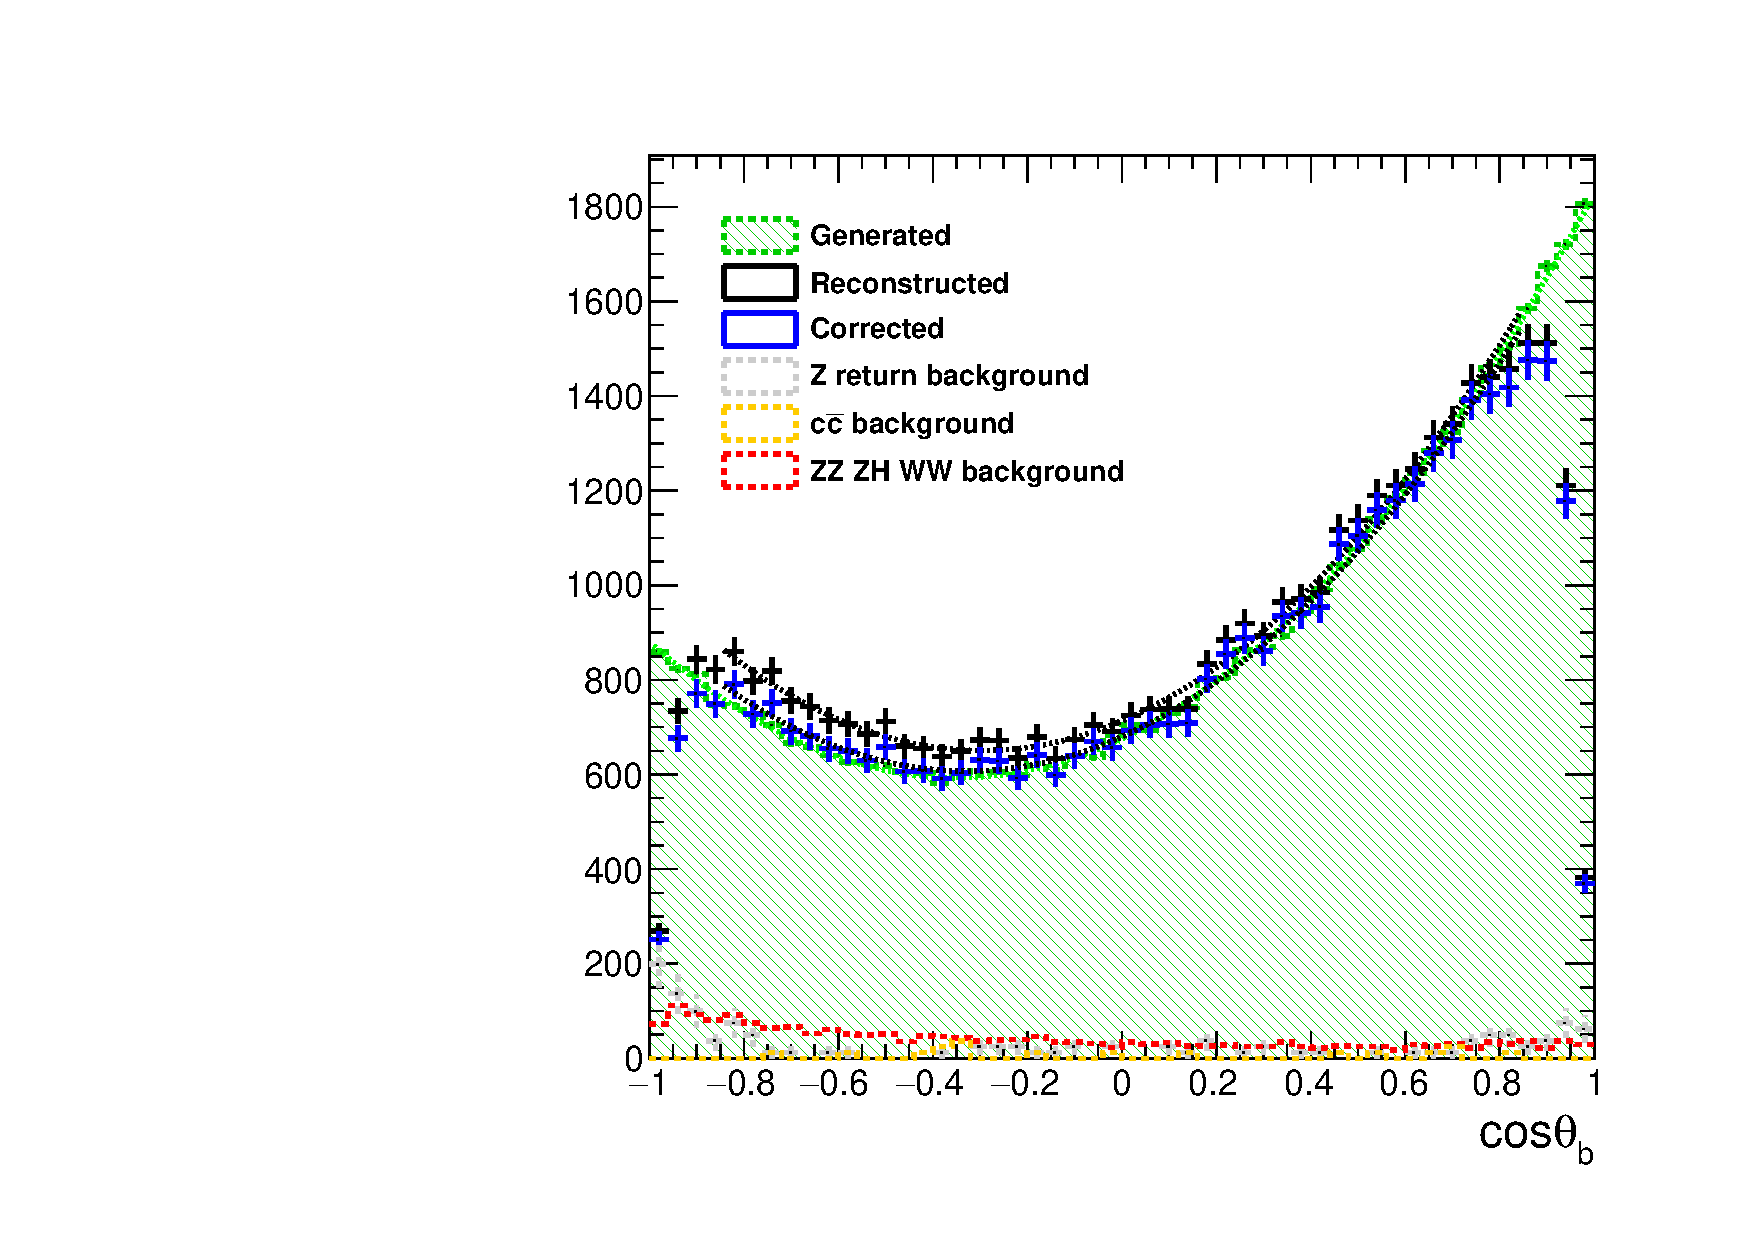
\includegraphics[width=0.45\linewidth]{./chapters/figures/basymmetry-final-right.pdf}
	\caption{Polar angle distribution $\cos{\theta_b}$ of generated $b$-quarks and final reconstructed 
         $b$-jets including any SM  background remaining after event selection. 
         Left:  $P(e^+,e^-)=(+100\%,-100\%)$ with a zoom of the region with negative 
         $\cos{\theta_b}$.
         Right: $P(e^+,e^-)=(-100\%,+100\%)$. From~\cite{Bilokin:2017lco}.  }
	\label{fig:ffbar_basym}
\end{figure*}


\begin{figure}
	\centering
	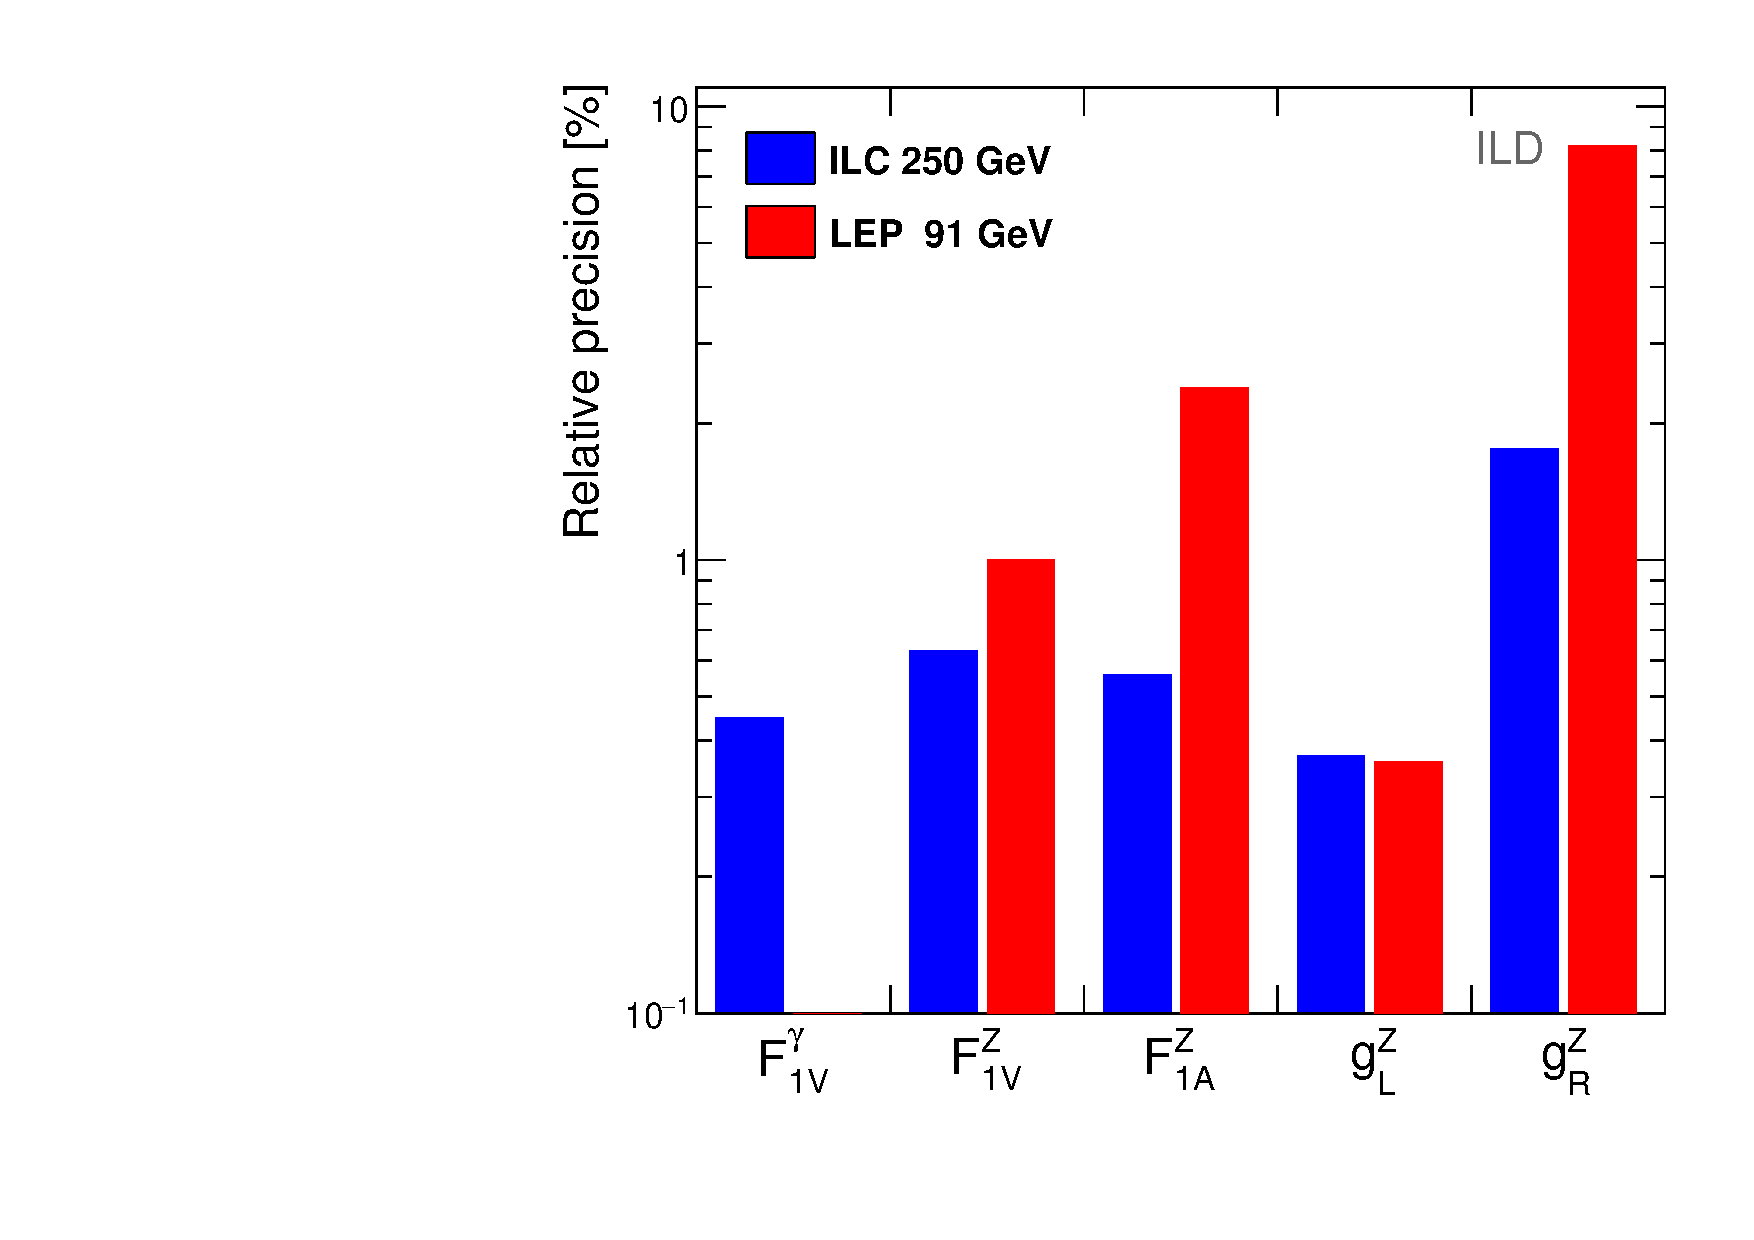
\includegraphics[width=0.95\columnwidth]{./chapters/figures/final-graph-ild.pdf}
	%	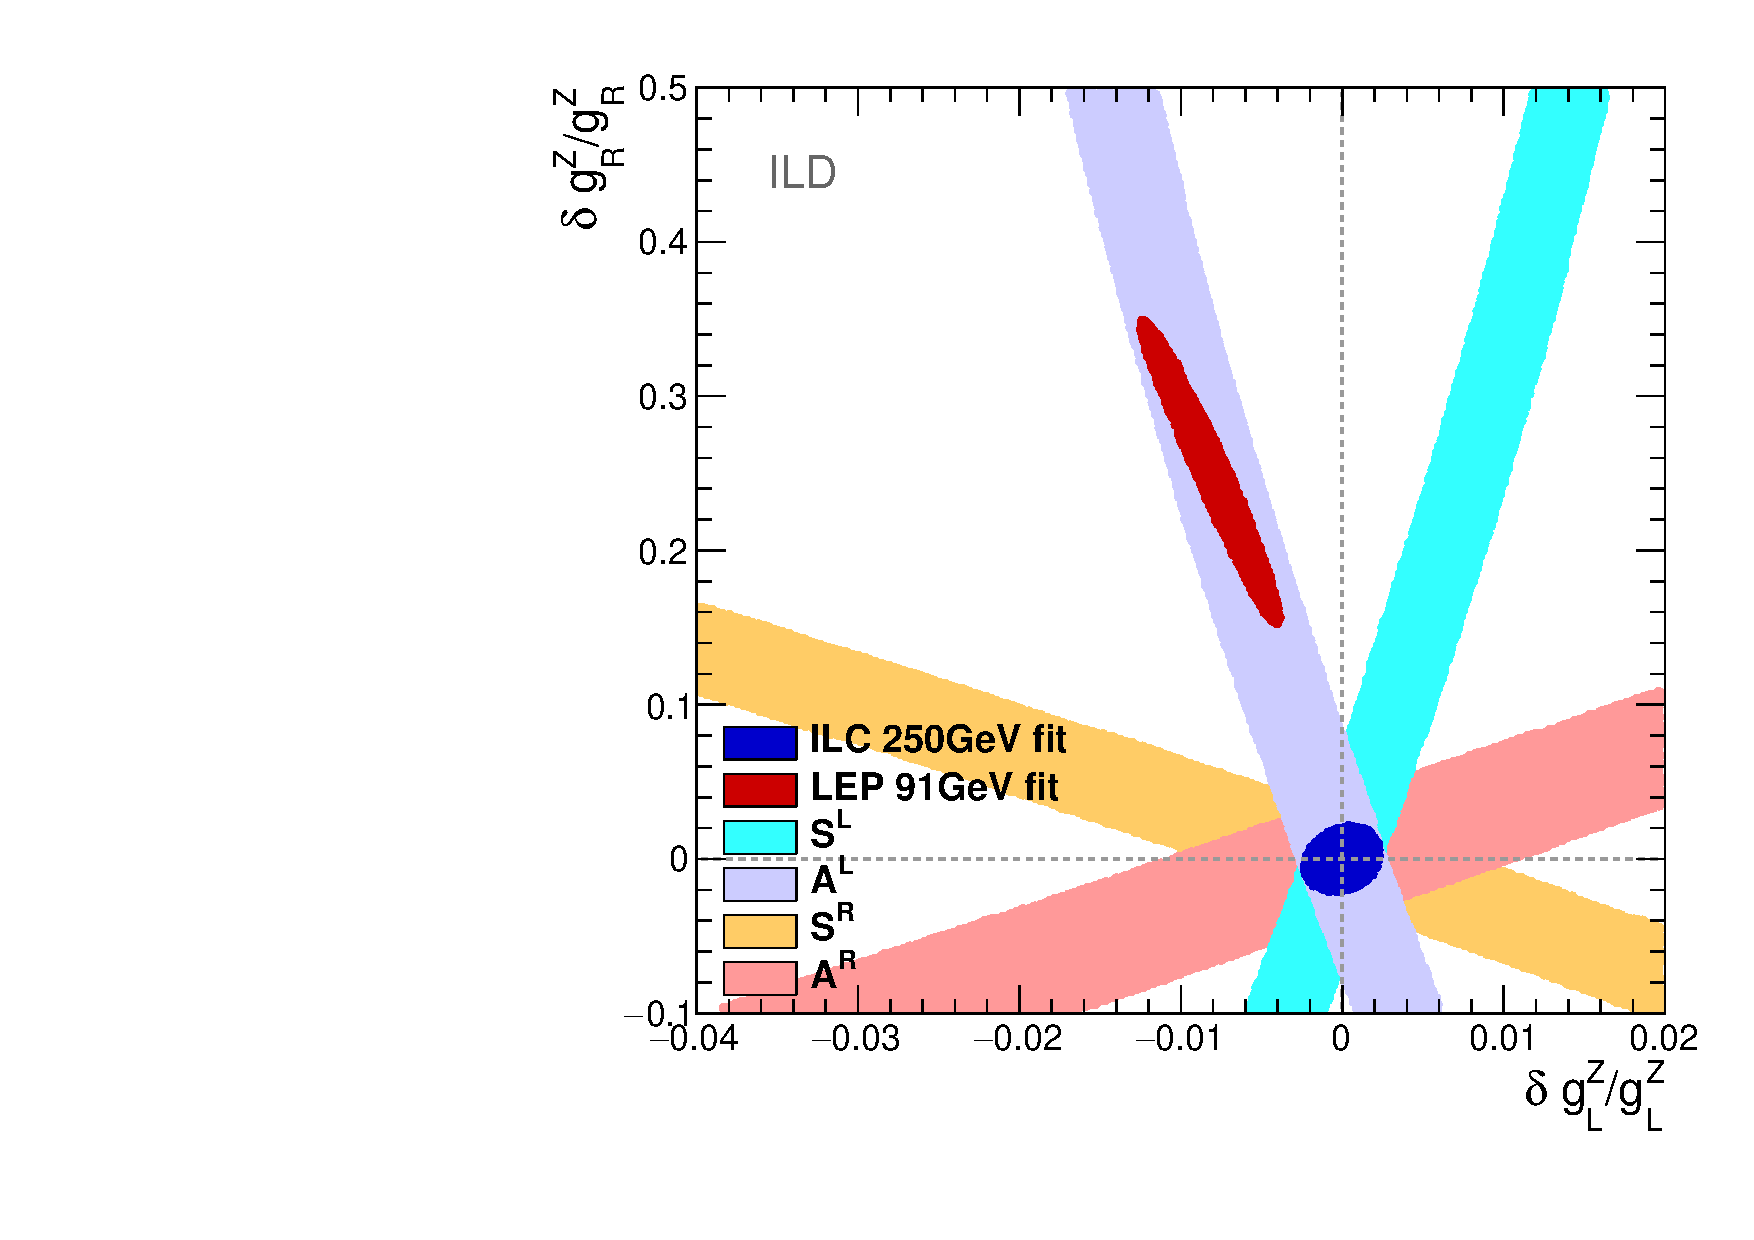
\includegraphics[width=0.95\linewidth]{./chapters/figures/ilc-precision-ild.png}
	\caption{\sl  Comparison of the LEP measurements to the expected 
                  precision at the ILC. The results of the ILC correspond to the 
                  integrated luminosity of $\mathcal{L}_I = 500$\,fb$^{-1}$ to be collected 
                   at $\sqrt{s} = 250$\,GeV before the luminosity upgrade. Final results for the
                  full 250\,GeV dataset would improve the precision further by about a factor of 2.
                   From~\cite{Bilokin:2017lco}.}
	\label{fig:LEPILCResult_3}
\end{figure}
